\documentclass[11pt,a4paper]{article}
\usepackage[margin=2.4cm]{geometry}
\usepackage[T1]{fontenc}
\usepackage{lmodern}
\usepackage{amsmath,amssymb}
\usepackage{booktabs}
\usepackage{graphicx}
\usepackage{siunitx}
\usepackage{microtype}
\usepackage{xcolor}
\usepackage{pgfplots}
\pgfplotsset{compat=1.18}
\usepgfplotslibrary{fillbetween}
\usepackage[hidelinks]{hyperref}
\sisetup{group-separator={,},group-minimum-digits=4}
\newcommand{\cfg}[1]{\texttt{#1}}
\setlength{\parskip}{0.3em}
\definecolor{s1}{HTML}{2a78d6}
\definecolor{s2}{HTML}{eb6834}
\definecolor{s3}{HTML}{1baf7a}
\definecolor{inkmuted}{HTML}{6b6a64}


\begin{document}

\begin{center}
  {\LARGE Sonar debris detector on a Raspberry Pi 4:\\[0.2em] on-device measurements}\\[0.6em]
  {\large Project report, \texttt{sonar\_edge}, milestone M5}\\[0.3em]
  10 November 2026
\end{center}
\vspace{0.5em}

\section*{Scope}

This report records the first measurements of the detector on the target
hardware, a Raspberry Pi~4. Four questions are addressed: (i) whether the
integer C runtime produces on the ARM processor exactly the output it
produces on the development laptop, so that the accuracy established by
cross-validation carries over unchanged; (ii) how long one frame takes, on
one core and on all four; (iii) how much memory and storage the program
needs; and (iv) how the cost compares with the crop classifier of the MCNN
paper that motivated the project. In the course of the measurement an
Advanced SIMD (NEON) kernel was added to the runtime, which made the
deployed model 6.2 times faster; its design and verification are included.
The data split, the network, the quantisation and the accuracy figures are
described in the companion report (\texttt{report/overview.pdf}) and are
summarised here only as far as needed.

\tableofcontents

\section{Hardware and software}
\label{sec:setup}

Table~\ref{tab:hw} lists the two machines. The laptop is where the runtime
was developed and where all earlier timings were taken; it serves as the
reference point. The Pi is a Raspberry Pi~4 Model~B (revision~1.5, 4~GB),
whose BCM2711 system-on-chip has four ARM Cortex-A72 cores at
\SI{1.8}{GHz}, \SI{32}{KB} of level-1 data cache per core and \SI{1}{MB} of
level-2 cache shared by the four cores. The Cortex-A72 implements the ARMv8.0
instruction set: it has the 128-bit Advanced SIMD (``NEON'') vector unit,
but not the 8-bit dot-product instructions (\texttt{sdot}/\texttt{udot})
introduced in ARMv8.2 and present on the Pi~5. Any vector kernel for the
Pi~4 must therefore be written with 16-bit multiplies.

\begin{table}[h]
\centering
\caption{Machines used. Both run the same source code; only the compiler target differs.}
\label{tab:hw}
\begin{tabular}{lll}
\toprule
 & Raspberry Pi 4 Model B & Laptop (reference) \\
\midrule
Processor & Broadcom BCM2711, 4 $\times$ Cortex-A72 & AMD Ryzen 5 5600H, 6 cores \\
Clock & \SI{1.8}{GHz} (governor \texttt{ondemand}) & up to \SI{4.2}{GHz} \\
Instruction set & AArch64, ARMv8.0 + NEON & x86-64 \\
Memory & 4 GB & 16 GB (14 GB usable) \\
Operating system & Debian 13 (Raspberry Pi OS), kernel 6.18 & Arch Linux \\
Compiler & gcc 14.2, native & gcc 16.2, native \\
Cooling & no fan (none registered by the OS) & laptop fan \\
\bottomrule
\end{tabular}
\end{table}

The runtime was copied to the Pi as source and built there with the
project's makefile, i.e.\ \texttt{gcc -std=c11 -O2 -Wall -Wextra -Werror
-pedantic}, with no other dependency than the C standard library. The
\texttt{-std=c11} flag (as opposed to \texttt{gnu11}) matters for
reproducibility: it disables the fusion of floating-point multiply and add
into one instruction, which the ARM compiler would otherwise apply and which
would change the last bits of the few floating-point operations in the box
decoder.

\section{Models under test}
\label{sec:models}

Four trained networks were measured, chosen to span the range of compute
studied in the project (Table~\ref{tab:models}). All four are the fold-0
models of the cross-validation, i.e.\ trained on the same frames, so the
test-fold accuracy column compares like with like. The pooled column is the
accuracy estimate for the configuration over all five folds, averaged over
seeds where more than one exists; it is the figure that describes the
configuration, while the test-fold column only identifies the particular
network that was run on the device.

\begin{table}[h]
\centering
\caption{Models measured on the Pi. MACs: multiply-accumulate operations per
frame. Fold-0 mAP: mAP@0.5 of the integer C runtime on the 439 frames of test
fold 0. Pooled mAP: 5-fold cross-validation, float, mean $\pm$ s.d.\ over
seeds (number of seeds in brackets).}
\label{tab:models}
\begin{tabular}{llrrrr}
\toprule
Model & Input & MACs & Parameters & Fold-0 mAP & Pooled mAP \\
\midrule
\cfg{small} (fallback) & $240 \times 160$ & 34.8 M & \num{42463} & 58.9 & 48.1 $\pm$ 1.1 (3) \\
\cfg{small} (\textbf{deployed}) & $360 \times 240$ & 78.4 M & \num{42463} & 63.8 & 52.6 $\pm$ 1.9 (3) \\
\cfg{small\_wide} & $360 \times 240$ & 203.5 M & \num{135359} & 68.1 & 56.9 $\pm$ 2.7 (3) \\
\cfg{wide} & $480 \times 320$ & 450.2 M & \num{172351} & 68.6 & 55.2 (1) \\
\bottomrule
\end{tabular}
\end{table}

\cfg{small} at $360 \times 240$ is the deployed configuration;
\cfg{small} at $240 \times 160$ was kept as a fallback in case the deployed
model proved too slow on the Pi; \cfg{small\_wide} at $360 \times 240$ is
the most accurate model found and was set aside as too expensive for the
device; \cfg{wide} is the largest model trained and marks the upper end of
the compute range.

\section{What is measured and how}
\label{sec:method}

\paragraph{Output equivalence.} The runtime is integer-only up to the final
box decoding, so it should produce the same output on any processor. This is
checked at three levels. (a)~The \emph{golden test} (\texttt{make test})
runs three frames through the network and compares all $45 \times 30 \times
15 = \num{20250}$ 32-bit values of the output map with values computed by the
Python integer reference; a single differing bit fails it. (b)~The
\emph{end-to-end test} runs the compiled program over all 439 frames of test
fold~0, copies the printed detections back to the laptop and scores them
with the same evaluation code and ground truth as the Python models. (c)~The
\emph{byte comparison} runs the laptop build of the same program on the same
439 frames and compares the two text outputs byte for byte, including the
six printed decimals of every score and box coordinate.

\paragraph{Latency.} The time for one frame, from the 8-bit image in memory
to the list of detections: the network and the decoder, i.e.\ the call
\texttt{se\_detect}. It excludes reading the file from disk, which in a
deployed system is replaced by the sonar driver. It is measured by the
command-line tool's benchmark mode, which calls \texttt{se\_detect}
repeatedly and reads the monotonic clock around each call. Ten frames spread
over the test fold are each processed 50 times, giving the mean over 500
calls; this is repeated three times. The three repeats differ by less than
1\% for every build except the NEON build of \cfg{wide} (3\%), so a
single mean is reported. The program runs on one core. The first frame
of each repeat pays for cold caches; with 500 calls this contributes well
under 1\%.

\paragraph{Throughput on four cores.} The runtime is single-threaded. The
simplest way to use the four cores is to run four independent copies, each
on its own stream of frames; this gives the throughput the board can sustain
when several sonar streams, or several frames of one stream, are processed in
parallel. Four copies are started together and the total number of frames
divided by the elapsed time gives frames per second. The per-copy latency
under this load is also recorded: it rises above the single-core value when
the copies compete for the shared level-2 cache and the memory bus.

\paragraph{Temperature and throttling.} The BCM2711 lowers its clock when the
die exceeds \SI{80}{\celsius} (soft limit) or \SI{85}{\celsius}. The firmware
reports the die temperature (\texttt{vcgencmd measure\_temp}) and a bit field
recording whether throttling or under-voltage has occurred since boot
(\texttt{vcgencmd get\_throttled}). Both were read before and after every
measurement; a throttled run would have been discarded.

\paragraph{Memory.} All buffers of the runtime are static arrays whose size is
fixed at compile time: two activation buffers that alternate as layer input
and output, the 32-bit output map and, for the NEON kernel, a 16-bit copy of
the weights. The program allocates nothing while running. The peak resident
memory of the whole process, which also counts the C library, the stack and
the program code, is read from the kernel (\texttt{VmHWM} in
\texttt{/proc/<pid>/status}) while the program is processing frames.

\paragraph{Program size.} The \texttt{text} segment reported by
\texttt{size}: machine code plus constant data, which includes the 8-bit
weights. This is what must be stored on the device.

\paragraph{Energy.} Not measured. The Pi~4 has no sensor for its own power
draw (the Pi~5 has one), and no external meter was available. The planned
method is an inline USB-C power meter or a current sensor on the
\SI{5}{V} supply: energy per frame is the increase of power over the idle
level, divided by the frame rate.

\section{Results}
\label{sec:results}

\subsection{Output equivalence on the device}

All three checks pass. The golden test passes on the Pi for all four models,
with the scalar and with the NEON kernel (Section~\ref{sec:neon}). Over the
439 test frames, the Pi printed \num{21333}, \num{25007}, \num{23218} and
\num{28096} detection lines for the four models of Table~\ref{tab:models},
and each output file is identical byte for byte to the laptop's. The scored
mAP is therefore identical too: 58.94, 63.81, 68.12 and 68.60\% on the Pi
and on the laptop. The NEON build's output over the full test fold is likewise
identical to the scalar build's (Section~\ref{sec:neon}).

The practical meaning is that no accuracy figure needs to be re-established
on the device. The Pi runs the same function as the Python integer
reference, whose accuracy was measured by cross-validation, and the
quantisation itself costs nothing measurable (52.3\% pooled int8 against
52.6\% float for the deployed model).

\subsection{Single-core latency, scalar code}
\label{sec:scalar}

Table~\ref{tab:latency} gives the latency of the original scalar runtime,
the one developed and timed on the laptop. The column ``GMAC/s'' divides the
model's multiply-accumulate count by the latency: it is the effective speed
of the inner loop and makes models of different size comparable.

\begin{table}[h]
\centering
\caption{Latency per frame, one core, \texttt{-O2}. Mean over 3 $\times$ 500
calls; the three repeats agree within 1\%.}
\label{tab:latency}
\begin{tabular}{lrrrrrr}
\toprule
 & & \multicolumn{2}{c}{Laptop, scalar} & \multicolumn{2}{c}{Pi 4, scalar} & \\
\cmidrule(lr){3-4}\cmidrule(lr){5-6}
Model & MACs & ms & GMAC/s & ms & GMAC/s & Pi/laptop \\
\midrule
\cfg{small} $240 \times 160$ & 34.8 M & 9.0 & 3.9 & 56.0 & 0.62 & 6.2 \\
\cfg{small} $360 \times 240$ & 78.4 M & 20.1 & 3.9 & 125.9 & 0.62 & 6.3 \\
\cfg{small\_wide} $360 \times 240$ & 203.5 M & 27.6 & 7.4 & 300.1 & 0.68 & 10.9 \\
\cfg{wide} $480 \times 320$ & 450.2 M & 54.8 & 8.2 & 656.0 & 0.69 & 12.0 \\
\bottomrule
\end{tabular}
\end{table}

On the Pi the scalar runtime executes 0.62--0.69 billion multiply-accumulates
per second, almost independently of the model, so latency is proportional to
the MAC count: 56~ms for the fallback, 126~ms for the deployed model, 0.66~s
for \cfg{wide}. The deployed model runs at 7.9 frames per second.

This is slower than the 70--100~ms projected before the measurement, which
had assumed a Pi-to-laptop ratio of 3--5. The measured ratio is 6.2 for the
32-channel models and 11--12 for the 64-channel ones. Clock frequency
accounts for a factor of about 2.3. The rest depends on what each compiler
makes of the plain C loop. Both compilers vectorise the inner dot product at
\texttt{-O2} (verified in the generated assembly), but with very different
results: on the 64-channel layers the laptop reaches 7--8~GMAC/s, while the
Pi stays at 0.7. The compilers also differ in version (gcc~16.2 against
14.2), and the reasons were not analysed further. What matters for
deployment is that the compiler does not deliver the vector unit's
throughput on the Pi, which motivated writing the vector code by hand.

\subsection{NEON kernel}
\label{sec:neon}

\paragraph{Design.} Nearly all of the work is in the $3 \times 3$
convolutions. For an output pixel the runtime computes, for every output
channel $o$,
\begin{equation}
  \mathrm{acc}_o = b_o + \sum_{t=1}^{9} \sum_{i=1}^{c_\text{in}} W_{o,t,i}\, x_{t,i},
  \label{eq:conv}
\end{equation}
where $t$ runs over the nine taps of the kernel, $x_{t,i} \in [0, 255]$ is
an 8-bit activation and $W_{o,t,i} \in [-127, 127]$ an 8-bit weight. The
scalar code evaluates this as one dot product over $i$ per output channel
and tap. The NEON kernel reorders the work so that 16 output channels are
computed at once. For each tap $t$ and input channel $i$, the single value
$x_{t,i}$ is multiplied by the 16 weights $W_{o..o+15,\,t,\,i}$ and added to
16 running sums held in four vector registers of four 32-bit lanes each.
The instruction that does this, \texttt{vmlal\_laneq\_s16}, multiplies four
16-bit weights by one 16-bit lane of another register and adds the four
32-bit products to an accumulator, so one instruction performs four of the
multiply-accumulates of Eq.~\eqref{eq:conv}. Eight consecutive input values
are loaded and widened from 8 to 16 bits with one instruction pair, and each
of the eight lanes is then used in turn. To make the 16 weights for a given
$(t, i)$ adjacent in memory, the weights are re-laid out once at start-up
from the stored order $[o][t][i]$ to $[t][i][o]$ and widened to 16 bits;
this copy is a static array of $9\, c_\text{in} c_\text{out}$ 16-bit values
per layer (83~KB for the deployed model). Vectorising over output channels
rather than input channels has two advantages: the first layer, which has a
single input channel, is vectorised as well as the others, and no horizontal
sum across vector lanes is needed at the end.

\paragraph{Why it is exact.} Every product $W x$ satisfies $|W x| \le 127
\cdot 255 = \num{32385} < 2^{15}$, and the 16-bit-by-16-bit multiply produces
it exactly as a 32-bit value. The sums are accumulated in 32-bit integers as
in the scalar code; integer addition is associative, so the different order
of summation cannot change the result, and the bound $|\mathrm{acc}| <
2^{28}$ established for the scalar runtime rules out overflow. The kernel is
therefore bit-identical to the scalar one by construction, not merely within
a tolerance. This is confirmed by the golden test on all four models and by
the full test-fold output, which is identical to the scalar output byte for
byte.

\paragraph{Four pixels per pass.} In the kernel as described, the 16 weights
for each $(t, i)$ are loaded from memory once per output pixel and used for
four instructions. A second version computes four horizontally adjacent
output pixels together: the same two weight registers are used against the
inputs of all four pixels, so each weight load now serves 16
multiply-accumulate instructions instead of four. This needs 16 accumulator
registers (four pixels $\times$ 16 output channels), two weight registers and
four input registers, which fits within the 32 vector registers of AArch64;
the generated code was checked to keep everything in registers. The products
and sums are the same as before, only grouped differently, so the argument
for exactness is unchanged. Pixels left over at the end of a row, and layers
whose input channel count is not a multiple of 8 (only the first layer, with
one input channel), use the single-pixel kernel.

\paragraph{Selection.} The NEON code is compiled when the target is AArch64
and is used for every layer whose number of output channels is a multiple of
16 (all layers of all four models). Other targets, such as the laptop,
compile the scalar code unchanged. \texttt{-DSE\_NO\_NEON} forces the scalar
path on the Pi and \texttt{-DSE\_NEON\_1PX} the single-pixel kernel, for
comparison. Together the two kernels add about 150 lines to the runtime.

\paragraph{Results.} Table~\ref{tab:neon} compares the builds of the
deployed model. Letting the compiler vectorise for the specific processor
(\texttt{-O3 -mcpu=cortex-a72}) gives a factor of 1.7; the hand-written
single-pixel kernel gives 5.6, compiler flags add nothing further to it
within the run-to-run spread, and the four-pixel kernel gives 6.2. The
default \texttt{-O2} build with the four-pixel kernel is the deployed one.
Table~\ref{tab:neonall} gives the gain for all four models. Every NEON
build passes the golden test, and the full test-fold output of every
four-pixel build is identical byte for byte to the scalar output.

\begin{table}[h]
\centering
\caption{Deployed model (\cfg{small}, $360 \times 240$), Pi~4, one core.
The single-pixel kernel was measured in two separate builds (22.5 and
22.1~ms); the first value is shown.}
\label{tab:neon}
\begin{tabular}{lrrr}
\toprule
Build & ms / frame & GMAC/s & vs.\ scalar \texttt{-O2} \\
\midrule
scalar, \texttt{-O2} & 125.9 & 0.62 & 1.0 \\
scalar, \texttt{-O3 -mcpu=cortex-a72} & 75.7 & 1.04 & 1.7 \\
NEON 1 pixel, \texttt{-O2} & 22.5 & 3.48 & 5.6 \\
NEON 1 pixel, \texttt{-O3 -mcpu=cortex-a72} & 21.5 & 3.65 & 5.9 \\
\textbf{NEON 4 pixels, \texttt{-O2}} & \textbf{20.3} & \textbf{3.85} & \textbf{6.2} \\
\bottomrule
\end{tabular}
\end{table}

\begin{table}[h]
\centering
\caption{Pi 4, one core, \texttt{-O2}, ms per frame. Speed-up, GMAC/s and
frames per second refer to the four-pixel kernel.}
\label{tab:neonall}
\begin{tabular}{lrrrrrr}
\toprule
Model & Scalar & NEON 1 px & NEON 4 px & Speed-up & GMAC/s & Frames/s \\
\midrule
\cfg{small} $240 \times 160$ & 56.0 & 10.2 & 9.0 & 6.2 & 3.88 & 112 \\
\cfg{small} $360 \times 240$ & 125.9 & 22.5 & 20.3 & 6.2 & 3.85 & 49 \\
\cfg{small\_wide} $360 \times 240$ & 300.1 & 77.6 & 46.5 & 6.4 & 4.37 & 21.5 \\
\cfg{wide} $480 \times 320$ & 656.0 & 140.9 & 91.8 & 7.1 & 4.91 & 10.9 \\
\bottomrule
\end{tabular}
\end{table}

With the single-pixel kernel the 32-channel models reach about
3.5~GMAC/s, but the two models with 64-channel layers only 2.6 and 3.2. The
16-bit weight table of a $64 \times 64$ layer is \SI{74}{KB} (against
\SI{18}{KB} for $32 \times 32$), more than the \SI{32}{KB} level-1 data
cache, so in the single-pixel kernel those weights are re-read from the
level-2 cache for every output pixel. The four-pixel kernel cuts that
traffic by four, and the result supports this explanation: the 64-channel
models gain the most from it (1.7 and 1.5 times, to 4.4 and 4.9~GMAC/s),
while the 32-channel models, whose weights fit in the level-1 cache, gain
only 11--13\%. With weight traffic reduced, the larger models now reach
the higher GMAC/s.
Cache misses were not measured directly, so this remains an inference from
the timings, though now one with a confirmed prediction.

Figure~\ref{fig:latency} summarises the latency of all builds against the
compute of the model.

\begin{figure}[h]
\centering
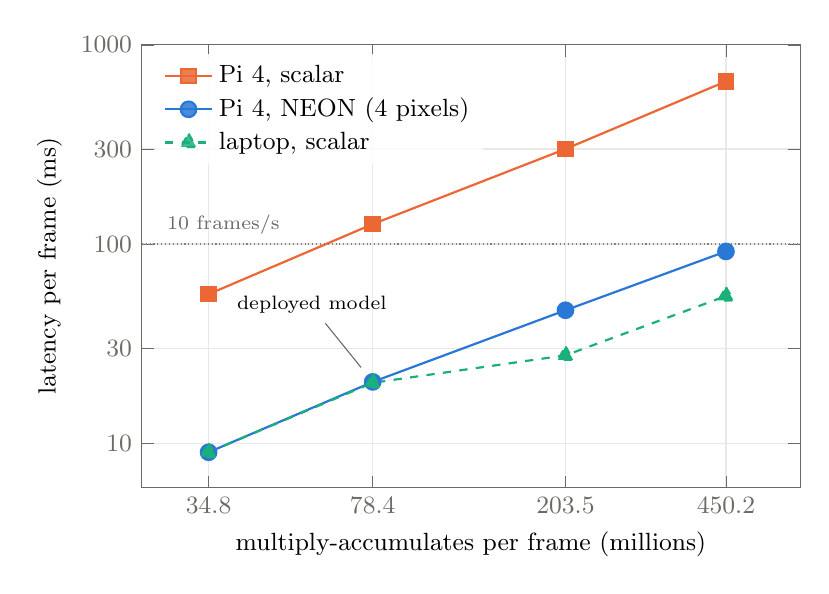
\begin{tikzpicture}
\begin{loglogaxis}[
  width=0.82\textwidth, height=7.2cm,
  xlabel={multiply-accumulates per frame (millions)},
  ylabel={latency per frame (ms)},
  xmin=25, xmax=650, ymin=6, ymax=1000,
  xtick={34.8,78.4,203.5,450.2}, xticklabels={34.8,78.4,203.5,450.2},
  ytick={10,30,100,300,1000}, yticklabels={10,30,100,300,1000},
  axis line style={inkmuted}, tick style={inkmuted},
  ticklabel style={font=\small, text=inkmuted}, label style={font=\small},
  grid=major, major grid style={gray!18},
  legend style={at={(0.02,0.98)}, anchor=north west, font=\small, draw=none, fill=white, fill opacity=0.85, text opacity=1},
  legend cell align=left,
]
\addplot[s2, thick, mark=square*, mark size=2.6pt] coordinates {(34.8,56.0) (78.4,125.9) (203.5,300.1) (450.2,656.0)};
\addlegendentry{Pi 4, scalar}
\addplot[s1, thick, mark=*, mark size=2.8pt] coordinates {(34.8,9.0) (78.4,20.3) (203.5,46.5) (450.2,91.8)};
\addlegendentry{Pi 4, NEON (4 pixels)}
\addplot[s3, thick, dashed, mark=triangle*, mark size=3.2pt] coordinates {(34.8,9.0) (78.4,20.1) (203.5,27.6) (450.2,54.8)};
\addlegendentry{laptop, scalar}
\addplot[gray, densely dotted] coordinates {(25,100) (650,100)};
\node[font=\scriptsize, text=inkmuted, anchor=south west] at (axis cs:27,100) {10 frames/s};
\draw[inkmuted] (axis cs:74,24) -- (axis cs:62,40);
\node[font=\scriptsize, anchor=south] at (axis cs:58,40) {deployed model};
\end{loglogaxis}
\end{tikzpicture}
\caption{Latency against compute, one core, logarithmic axes. The four points
of each line are the four models of Table~\ref{tab:models}. A line of slope 1
means constant GMAC/s. The dotted line marks \SI{100}{ms}, i.e.\ 10 frames
per second. The two leftmost Pi NEON points coincide almost exactly with the
laptop's scalar points.}
\label{fig:latency}
\end{figure}

\subsection{Throughput on four cores and temperature}

Table~\ref{tab:throughput} gives the frame rate with four copies of the
program running at once, and the temperature reached.

\begin{table}[h]
\centering
\caption{Four copies in parallel, one per core. ``Per copy'' is the mean latency
of each copy under this load (range over the four copies). Temperature at the end
of the run. $^{*}$The firmware recorded that the soft temperature limit
(\SI{80}{\celsius}) was reached during this run; see text. The firmware flag
is cumulative until reboot, so it cannot tell whether later runs (the NEON
rows of \cfg{wide} and all four-pixel rows) were throttled; their
temperatures stayed below the limit.}
\label{tab:throughput}
\begin{tabular}{llrrrr}
\toprule
Model & Kernel & 1 core, ms & 4 cores, per copy, ms & Frames/s & End temp. \\
\midrule
\cfg{small} $240 \times 160$ & scalar & 56.0 & 56.4--56.6 & 70.6 & \SI{72.0}{\celsius} \\
                              & NEON 1 px & 10.2 & 10.7--11.8 & 339 & \SI{60.3}{\celsius} \\
                              & NEON 4 px & 9.0 & 9.3--9.4 & 425 & \SI{58.9}{\celsius} \\
\cfg{small} $360 \times 240$ & scalar & 125.9 & 126.7--126.9 & 31.4 & \SI{68.6}{\celsius} \\
                              & NEON 1 px & 22.5 & 25.6--26.8 & 149 & \SI{65.7}{\celsius} \\
                              & NEON 4 px & 20.3 & 21.0--21.3 & 187 & \SI{64.2}{\celsius} \\
\cfg{small\_wide} $360 \times 240$ & scalar & 300.1 & 302.6--303.8 & 13.2 & \SI{75.9}{\celsius} \\
                              & NEON 1 px & 77.6 & 161.5--163.8 & 24.4 & \SI{71.5}{\celsius} \\
                              & NEON 4 px & 46.5 & 59.1--59.5 & 67.1 & \SI{72.0}{\celsius} \\
\cfg{wide} $480 \times 320$ & scalar & 656.0 & 663.2--664.8 & 6.0 & \SI{81.8}{\celsius}$^{*}$ \\
                              & NEON 1 px & 140.9 & 252.7--261.3 & 15.3 & \SI{78.4}{\celsius} \\
                              & NEON 4 px & 91.8 & 100.5--101.5 & 39.4 & \SI{78.8}{\celsius} \\
\bottomrule
\end{tabular}
\end{table}

The scalar code scales perfectly to four cores: each copy is as fast as when
alone. With the single-pixel NEON kernel the 32-channel models lost 5--15\%
per copy and the 64-channel models about half, so that four copies of
\cfg{small\_wide} were only 1.9 times as fast as one. This is the same weight
traffic as above, now competing for the \SI{1}{MB} level-2 cache and the
memory bus shared by the four cores. The four-pixel kernel largely removes
it: per-copy slowdown is 3--5\% for the 32-channel models and 10--28\% for the
64-channel ones, and four cores give 3.8 times the single-core rate for
the 32-channel models (187 frames per second for the deployed model) and
3.1--3.6 times for the 64-channel models.

Without a fan, every run of the three smaller models stayed at or below
\SI{76}{\celsius}. The four-copy scalar run of \cfg{wide}, the longest run
at full load (about two minutes), reached \SI{81.8}{\celsius}, and the
firmware recorded that the soft temperature limit had been reached, at which
the BCM2711 begins to lower its clock. The effect on that run was small (664
against 656~ms per frame), but it shows that sustained four-core operation
of the heavier models needs a heat sink or fan; the deployed model at four
cores ran at \SI{64}{\celsius}.

\subsection{Memory and program size}

\begin{table}[h]
\centering
\caption{Static buffers (bss), program code and constants (text), and peak
resident memory of the whole process, NEON build. The scalar build has the
same text and 83--344~KB less bss (no 16-bit weight copy).}
\label{tab:memory}
\begin{tabular}{lrrr}
\toprule
Model & Static buffers & Code + weights & Peak resident \\
\midrule
\cfg{small} $240 \times 160$ & 429 KB & 53 KB & 1.8 MB \\
\cfg{small} $360 \times 240$ & 854 KB & 53 KB & 2.3 MB \\
\cfg{small\_wide} $360 \times 240$ & 1034 KB & 145 KB & 2.6 MB \\
\cfg{wide} $480 \times 320$ & 1699 KB & 181 KB & 3.4 MB \\
\bottomrule
\end{tabular}
\end{table}

The deployed model needs \SI{2.3}{MB} of memory in total, of which the
largest part is the two activation buffers of \SI{355}{KB} each, sized for
the first layer's output. The program file is \SI{54}{KB}, of which \SI{42}{KB}
are the weights. Memory is not a constraint on any Raspberry Pi; these
figures would also fit a microcontroller-class device with a few megabytes
of RAM, although the latency there would be a separate question.

\subsection{Comparison with the MCNN crop classifier}

The MCNN of the paper that motivated this project classifies one object crop
at a time. Its input is the crop zero-padded to $305 \times 305$, and it has
2.8~M parameters; counting the operations of our reimplementation gives
234.7~M multiply-accumulates per crop. The dataset has on average 2.08
annotated objects per frame (\num{3882} boxes in \num{1868} frames, the
\emph{Wall} class included), so classifying the objects of one frame costs
about 490~M multiply-accumulates. This is classification only: the crops
must be found first, and the paper takes them from the manual annotations.
The deployed detector finds and classifies all objects of a frame in one
pass of 78.4~M multiply-accumulates, about one sixth of MCNN's
classification cost, with 66 times fewer parameters (\num{42463} against 2.8~M).
The paper's claim that MCNN is suited to embedded use was not supported by a
measurement; the figures above give the comparison in operation counts, and
the deployed detector's measured latency on the Pi is 20.3~ms per frame.

\section{Discussion}

\paragraph{The deployed model is fast enough.} With the NEON kernel the
deployed model processes a frame in 20.3~ms on one core, 49 frames per
second. Forward-looking imaging sonars of the class that recorded the
dataset typically deliver on the order of 10--15 frames per second, so one
core keeps up with the sensor with a factor of three or more to spare, and
the other three cores remain free for the rest of the system. The
$240 \times 160$ fallback is no longer needed for speed.

\paragraph{The accuracy reference becomes a candidate.} \cfg{small\_wide} at
$360 \times 240$ is the most accurate configuration found (56.9 against 52.6
pooled mAP over three seeds each, ahead in every seed pairing and every fold,
Table~\ref{tab:models}). A 48-channel variant in between (132~M MACs) gave
no measurable gain at one seed (50.9), so there is no cheaper intermediate
model to choose instead.
It had been ruled out on cost. On the Pi it now runs at 46.5~ms per frame,
21.5 frames per second on one core, which is above the sensor rate quoted
above. Whether to deploy it is a trade-off between about four points of mAP
and a factor of 2.6 in compute (2.3 in measured time, and presumably in
energy); the choice depends on the power budget of the vehicle, which the
energy measurement would settle.

\paragraph{Design choices confirmed.} The decision to write the runtime in
plain C with integer arithmetic and no library is what makes the
equivalence result possible: the program on the Pi is verifiably the same
function as the one evaluated in Python, so no accuracy is lost or needs to
be re-measured in deployment. The decision to defer vector code until the
target was measured is also borne out: the scalar Pi measurement showed that
the compiler alone recovers only a factor of 1.7, the hand-written kernel
was then targeted at the specific instruction set of the Pi~4, and the
measured weakness of its first version on the 64-channel layers pointed
directly to the four-pixel variant.

\section{Limitations}

\begin{itemize}
  \item Energy per frame was not measured (no power sensor on the Pi~4, no
  external meter); this is the remaining item of the M5 plan.
  \item Thermal behaviour was observed over runs of one to three minutes on
  a board without a fan; the heaviest run reached the soft temperature
  limit. Sustained four-core operation, and operation inside
  a sealed housing as on an underwater vehicle, were not tested.
  \item Latency excludes the acquisition of the frame and its conversion to
  the $8$-bit Cartesian image the network expects; on a vehicle this is done
  by the sonar's software and its cost depends on the sensor interface.
  \item The cache explanation for the behaviour of the 64-channel layers is
  supported by the effect of the four-pixel kernel but was not confirmed by
  counting cache misses.
  \item Only a Pi~4 was measured. On a Pi~5 (Cortex-A76, \SI{2.4}{GHz},
  8-bit dot-product instructions) a dedicated kernel using \texttt{udot}
  would be expected to be several times faster again; this has not been
  tested.
  \item The MCNN comparison is in operation counts, not measured time;
  MCNN was not ported to the runtime.
\end{itemize}

\section{Summary}

\begin{itemize}
  \item On a Raspberry Pi~4 the C runtime produces output identical, byte for
  byte, to the laptop and bit for bit to the Python integer reference. The
  accuracy of the deployed model (52.6\% pooled mAP, 63.8\% on test fold 0)
  therefore holds on the device without re-measurement.
  \item A NEON kernel for the Pi~4's Cortex-A72, exact by construction and
  computing four output pixels per pass over the weights, makes the deployed
  model 6.2 times faster: 20.3~ms per frame (49 frames per second) on one
  core, against 126~ms for the original scalar code and 76~ms for the best
  the compiler achieves alone.
  \item Four cores process 187 frames per second of the deployed model at
  \SI{64}{\celsius} without a fan; only the heaviest model at full load
  reached the soft temperature limit. The process needs 2.3~MB of memory and a 54~KB
  program file.
  \item The most accurate model, \cfg{small\_wide} at $360 \times 240$, runs
  at 21.5 frames per second on one core (46.5~ms) and is now a deployment
  candidate.
  \item Open: energy per frame with an external meter; a sustained thermal
  test; a Pi~5 kernel using the dot-product instructions.
\end{itemize}

\end{document}
